\documentclass[oneside,12pt]{memoir}

\usepackage{mathptmx}  
\DoubleSpacing         
\usepackage{pwasu}  

\bibliographystyle{plain}


\usepackage[english]{babel}
\usepackage{amssymb,amsmath,graphicx,mdwlist,paralist,multirow,array,color,subfig}
\usepackage[noend]{algpseudocode}
\usepackage{chngpage,url,algorithm,algorithmicx,wrapfig}

\newcommand{\tab}{\hspace*{2em}}
\renewcommand{\algorithmicforall}{\textbf{for each}}

\DoubleSpacing

\begin{document}

\maxtocdepth{subparagraph} % put everything into the ToC
\pagestyle{plain}  % pagestyle for the prelims
\frontmatter
\thetitlepage

\setcounter{page}{1}
\asuabstract 
It is commonly known that High Performance Computing (HPC) systems are most frequently used by multiple users for batch job, parallel computations. Less well known, however, are the numerous HPC systems servicing data so sensitive that administrators enforce either \begin{inparaenum}[\itshape a\upshape)] 
\item sequential job processing - only one job at a time on the entire system, or
\item physical separation - devoting an entire HPC system to a single project until recommissioned.
\end{inparaenum}
The driving forces behind this type of security are numerous but share the common origin of data so sensitive that measures above and beyond industry standard are used to ensure information security. This paper presents a network security solution that provides information security above and beyond industry standard, yet still enabling multi-user computations on the system. This paper's main contribution is a mechanism designed to enforce high level time division multiplexing of network access (Time Division Multiple Access, or TDMA) according to security groups. By dividing network access into time windows, interactions between applications over the network can be prevented in an easily verifiable way. 

\asuacknowledgements
{I would like to acknowledge and thank Dr. Gupta for taking a chance and inviting me to work in Impact Lab, Dr. Varsamopoulos for his immense technical guidance (especially regarding Linux), and Dr. Ball for his earnest support of this thesis and its goals. I am intellectually and personally indebted to the members of Impact Lab for their help with the myriad of tasks that arose during my time with the lab. Special mention must go to Dr. Tridib Mukherjee, Dr. Ayan Bannerjee, and (soon to be Dr.) Zahra Abbasi for helping me with their seemingly boundless knowledge of the research we did, as well as Robin Gilbert for being a true friend and great colleague. I thank Raytheon for their capital support of our research. Finally, I thank my parents and brother for their love and support.
}

	\newpage
\vspace*{\fill}
\begingroup
\hspace*{\fill}
\centering{\textit{To my wife, Sara, for her unwavering support}}
\hspace*{\fill}
\endgroup
\vspace*{\fill}

\tableofcontents

\listoffigures

\mainmatter
\pagestyle{asu} 

\addtocontents{toc}{
 \protect\noindent CHAPTER \protect\par

}
\chapter{Introduction}
\label{chap:introduction}
High Performance Computing (HPC) systems consist of numerous individual computing systems networked and administrated together such that they can be used as a single system. Examples of these systems from popular culture include custom made models such as the Cray I (historically one of the first systems deemed HPC) and the modern IBM Blue Gene~\cite{leavitt2012big}. More common examples are simple Computer Clusters such as Beowulf clusters in which Commercial Off The Shelf (COTS) equipment is utilized~\cite{buyya1999high}. These latter systems are simple enough that they are frequently implemented by single users within hobbyists' homes~\cite{brown2004engineering}. Figures~\ref{fig:beowulf}~, \ref{fig:crayi}, and \ref{fig:blue_gene} show examples of these systems.

\begin{figure}
\centering
\begin{minipage}{4cm}
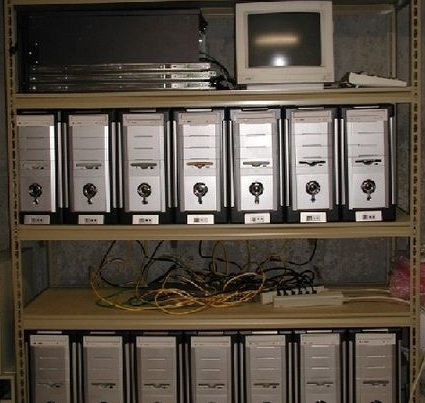
\includegraphics[width=4cm]{beowulf.jpg}
\caption{A beowulf cluster.~\cite{beowulf}}
\label{fig:beowulf}
\end{minipage}
\hspace{1em}
\begin{minipage}{4cm}
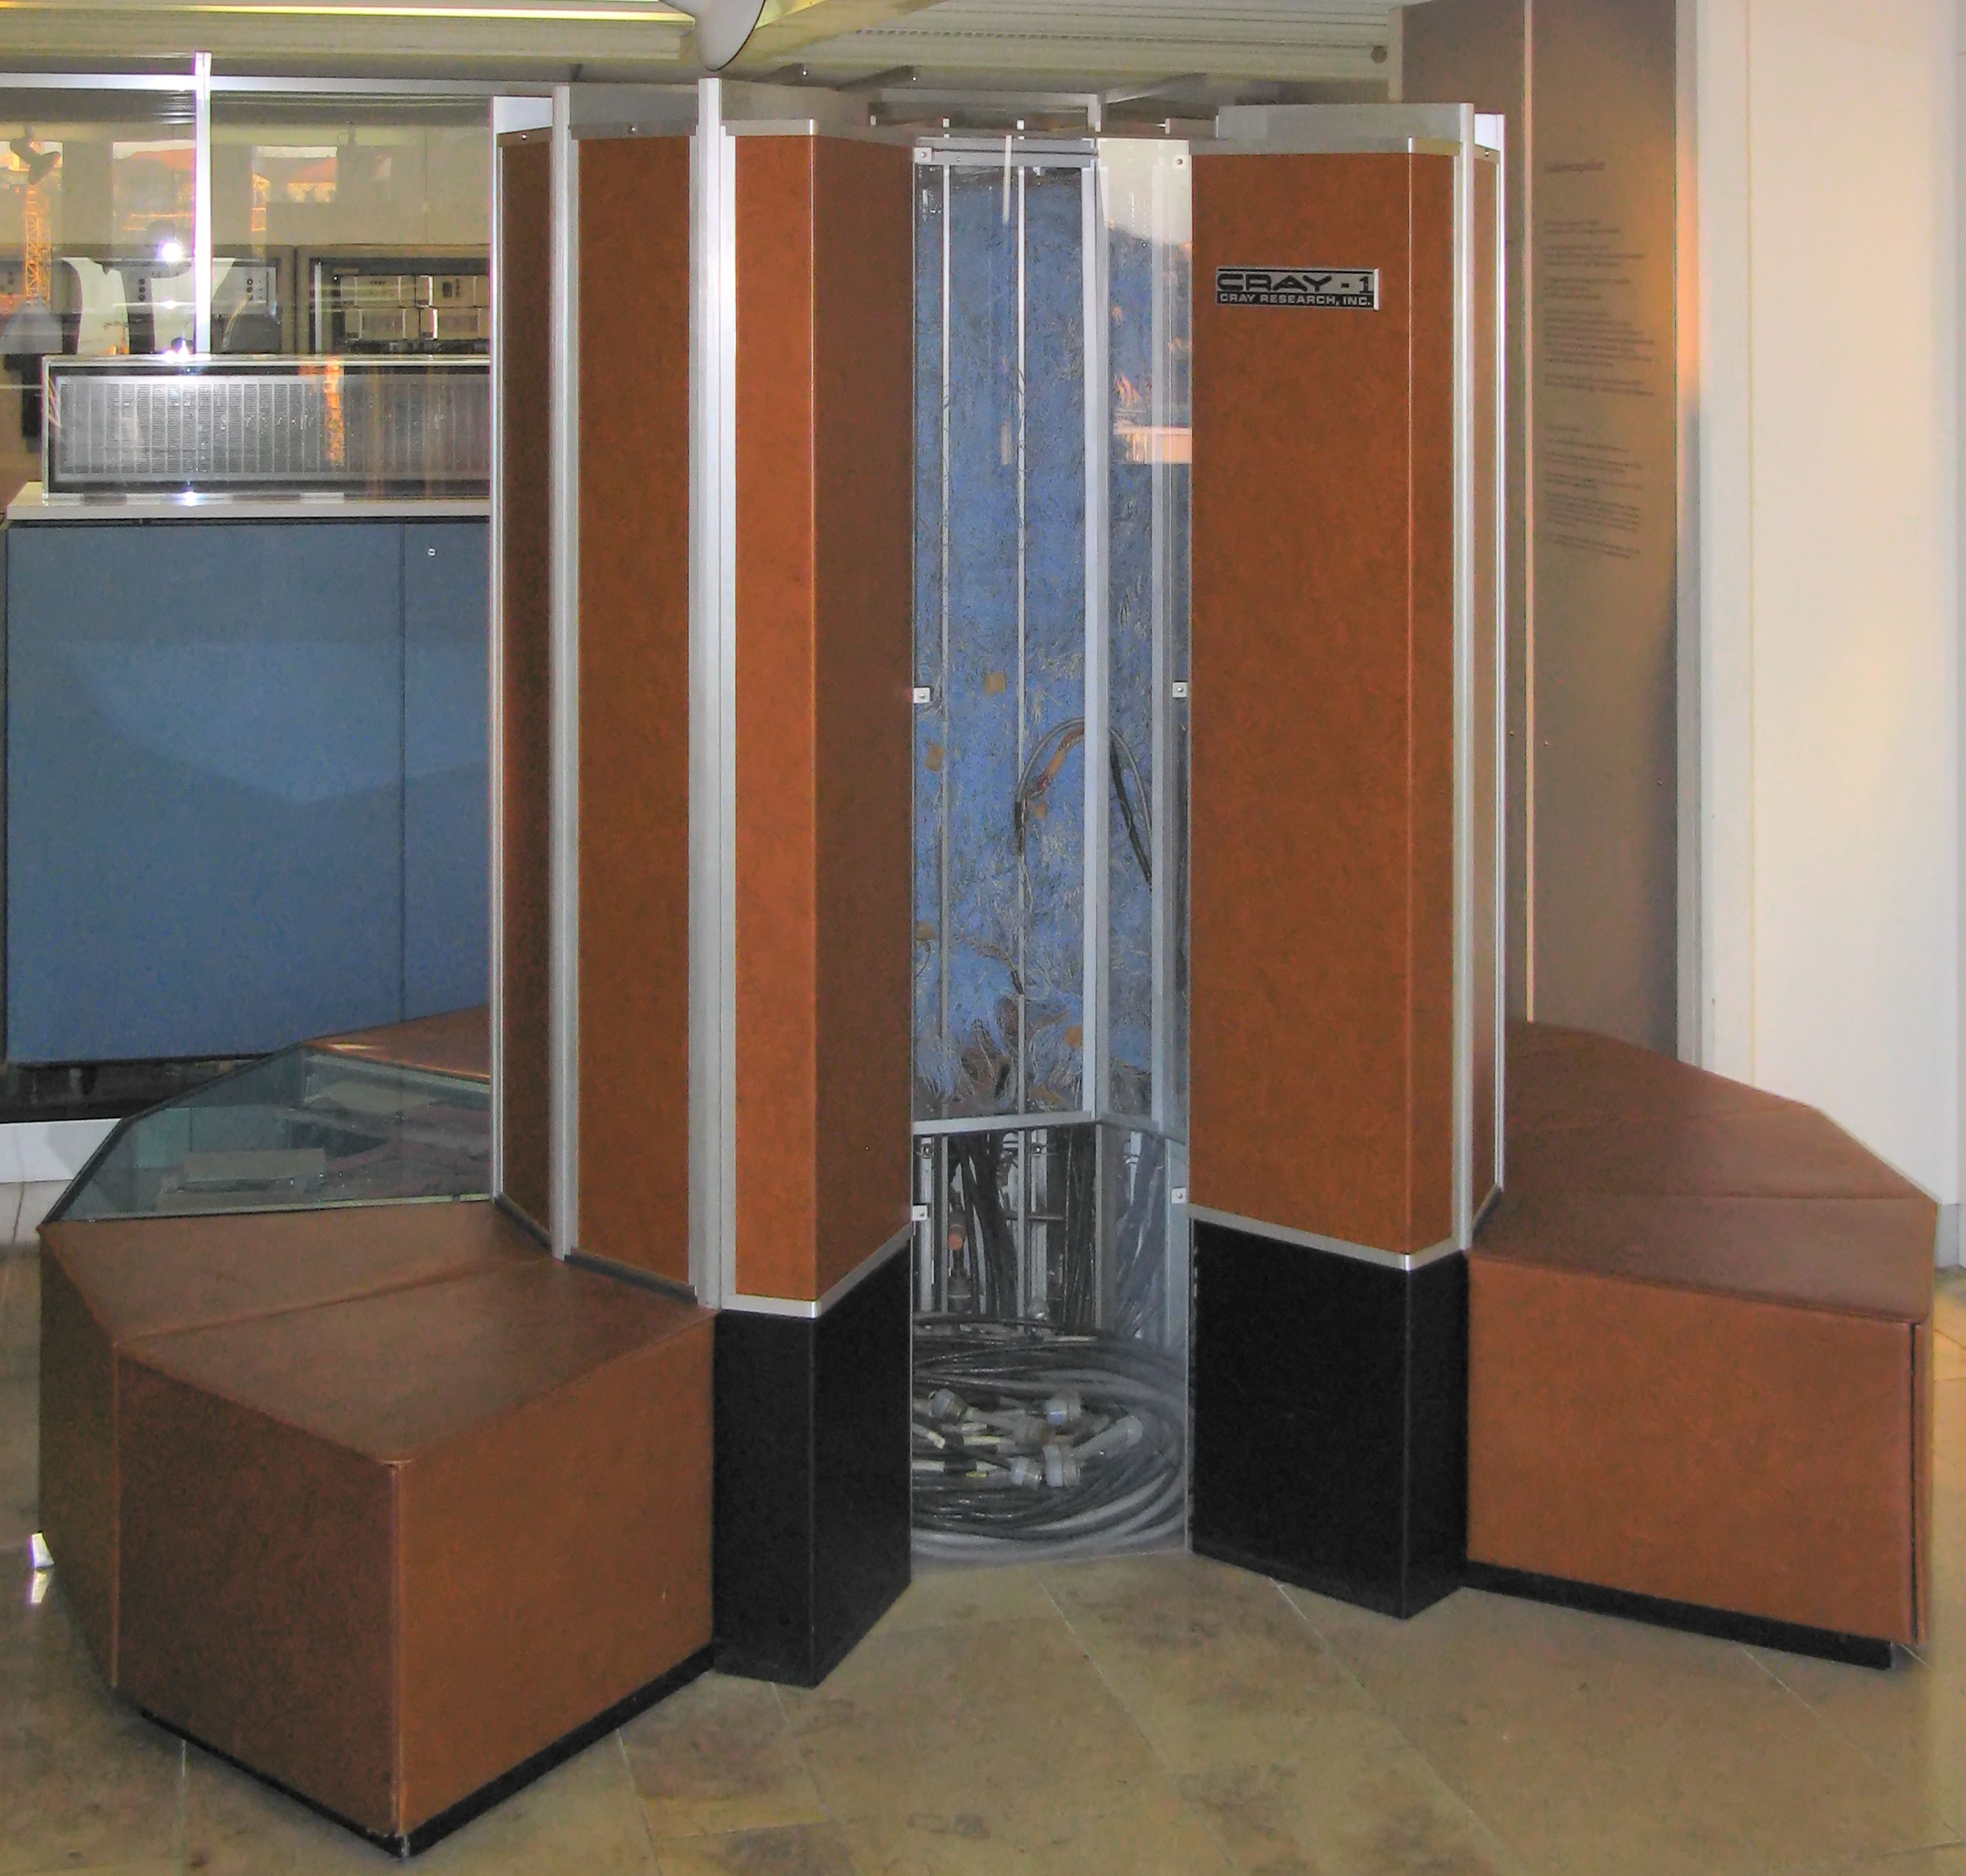
\includegraphics[width=4cm]{crayi.jpg}
\caption{The Cray I.~\cite{crayi}}
\label{fig:crayi}
\end{minipage}
\hspace{1em}
\begin{minipage}{4cm}
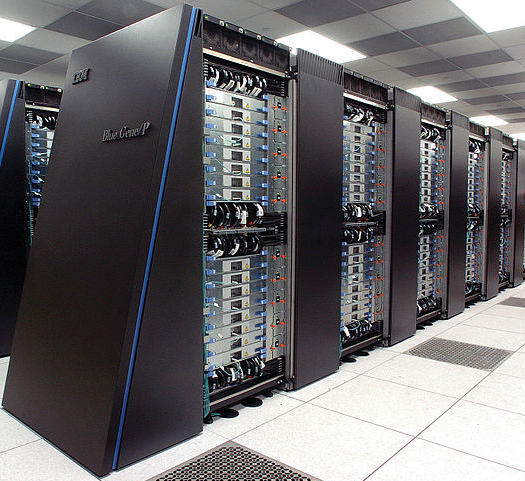
\includegraphics[width=4cm]{blue_gene.jpg}
\caption{IBM's Blue Gene.~\cite{blue_gene}}
\label{fig:blue_gene}
\end{minipage}
\end{figure}

\begin{figure}
\centering
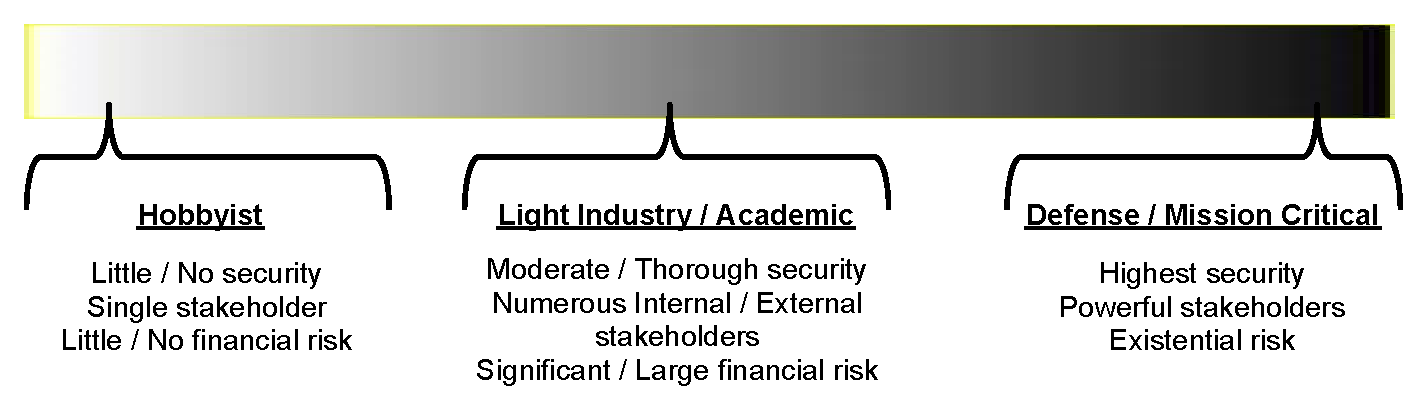
\includegraphics[scale=0.6]{security_spectrum.pdf}
\caption{The spectrum of environmental security requirements based on uses and stakeholders.}
\label{fig:security_spectrum}
\end{figure}
\section{Security Concerns}
Application developers for these systems span a broad spectrum, ranging from undergraduate students learning concurrent programming to defense contractors executing classified simulations. Key characteristics of this spectrum are shown in Figure~\ref{fig:security_spectrum}. Moving towards the most demanding end of the spectrum, security concerns among application-side stakeholders increase substantially and additional methods are employed to enforce information security. At some point along this spectrum stakeholders demand physical separation of the system from other users during operation to satisfy security concerns. The reasons behind this can be numerous, but stem from two major goals: simplicity of implementation and verification; and risk aversion/management. In the defense industry particularly, information security breaches can threaten the existence of entire programs due to certification revocation from agencies such as the Department of Defense (DoD)~\cite{classified_manual}, the DoD's Defense Security Service (DSS) agency~\cite{updatedclearing}, and the National Institute of Standards and Technology (NIST). Such risk reasonably implies physical separation of systems under operation from other users as well as numerous other physical security requirements. 

It is undeniable that physical separation provides a level of information security that is difficult to replicate through the use of software, however the financial costs are significant - devoting entire HPC systems to a single project, or running jobs sequentially with downtime for data cleansing between~\cite{updatedclearing}. 

\section{Time Division Multiple Access Scheme}
\label{sec:TDMA_intro}
This paper presents a Time Division Multiple Access (TDMA) scheme of network access as a viable alternative to physical separation. By modulating network access between application security groups we can provide an intuitive security mechanism, verifiable in real-time, capable of mimicking aspects of the security provided by physical separation. Furthermore by implementing this mechanism at the operating system level it becomes transparent to user applications, meaning no modification to existing application code is necessary. Providing a mechanism for operating multiple user applications on a single HPC system securely with the support of stakeholders can provide substantial monetary savings and efficiency gains over physical separation.

The scheme works by inserting gates to network access at each computing node (computing devices devoted to executing user applications) within the system. These gates are modulated open and closed by a central administrative program, denoted as the \textit{control server}, using knowledge of users and the data they own, denoted as \textit{security groups}. The key operation of the scheme is the control server modulating network access of individual computing nodes such that systems executing application(s) from one security group never have access at the same time as systems containing data from a different security group.

\begin{figure}
\centering
\begin{minipage}{6.5cm}
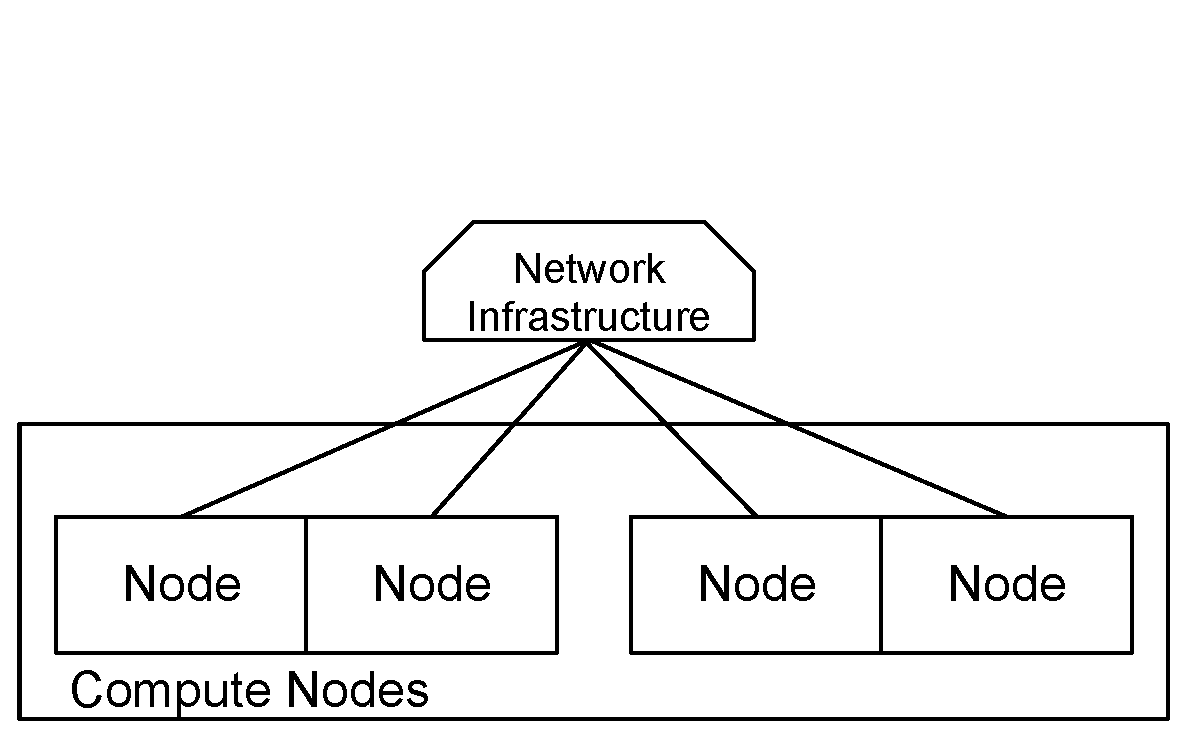
\includegraphics[width=6.5cm]{Simple_TDMA_Introduction_pt1.pdf}
\caption{Unmodified computing nodes.}
\label{fig:simple_TDMA_introduction_pt1}
\end{minipage}
\hspace{1em}
\begin{minipage}{6.5cm}
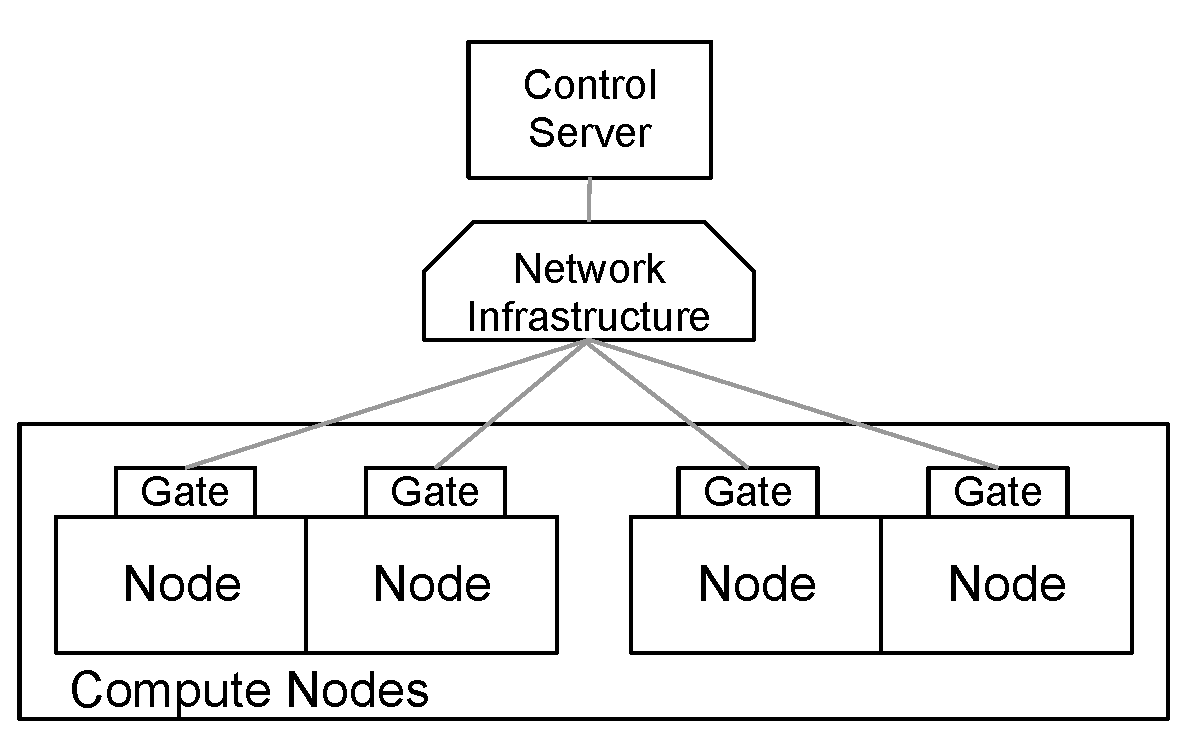
\includegraphics[width=6.5cm]{Simple_TDMA_Introduction_pt2.pdf}
\caption{TDMA overlaid onto Figure~\ref{fig:simple_TDMA_introduction_pt1}}
\label{fig:simple_TDMA_introduction_pt2}
\end{minipage}
\end{figure}

Chapter~\ref{chap:implementation} provides details on the implementation of this scheme, and Chapter~\ref{chap:tdma}: Section~\ref{sec:formal_definition} formally defines the scheme's operations.
\chapter{Related Work}
The problem statement and proposed solution represent the intersection of two somewhat disparate fields - Time Division Multiple Access and High Performance Computing Security. Related works are therefore divided between the two. 
\section{High Performance Computing Security}
The size and cost of HPC environments dictates that each system is somewhat unique. The security solutions implemented within each are similarly unique. Sandholm et al.~\cite{sandholm2004ogsa} make an attempt at rectifying this larger problem by creating a framework that automates user access permissions and resource allocation using "XACML (eXtensible Access Control Markup Language)". They further extend their solution by tying it in to existing job submission tools (Globus Toolkit~\cite{globus_toolkit} and NorduGrid~\cite{nordugrid}). 

Allcock et al.~\cite{allcock2001secure} developed a high-speed data transport protocol, GridFTP, as well as a corresponding administrative service providing for the creation, registration, and secure transportation of scientific computing datasets. For efficient execution, HPC applications must carefully consider characteristics of the data set under operation such as file size statistics, data creation/consumption rates, and logical distribution~\cite{chervenak2000data}. GridFTP implements management of these characteristics while maintaining customizable security using the authentication mechanisms defined in RFC 2228 "FTP Security Extensions"~\cite{horowitz1997ftp}. This solution, while useful in most scientific computing setting, still allows for application data, albeit encrypted, to be visible over the network to other user applications. This visibility renders it insufficient for the requirements of customers with the most stringent data security needs.
\section{Time Division Multiple Access}
Mages and Feng~\cite{mages1999method} patented a similar control scheme of computing resources via a centralized controller over the network. Their scheme, however, specifies only local media resources of the node as under the control of the central administrative node. Furthermore, their patent is intended for a much wider distributed use as digital rights management and security in consumer media devices, rather than our work on security in HPC environments.

\chapter{Problem Definition}
\label{chap:problem_definition}
We begin by defining an abstract HPC environment through which the general case of our security challenge is shown. In this section we provide brief descriptions of the major resources common to most HPC systems. Furthermore, to design our mechanism, certain assumptions must be made on how each resources is operated. 

\section{Assumptions on the Computing Environment}
\begin{figure}
\centering
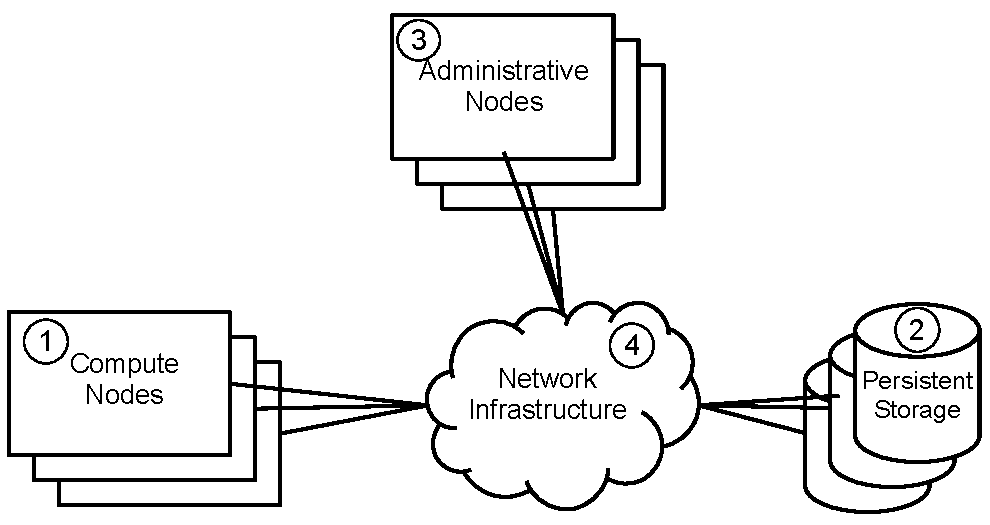
\includegraphics[scale=0.7]{abstract_hpc_environment.pdf}
\caption{An abstract HPC environment.}
\label{fig:abstract_hpc_environment}
\end{figure}
There are four basic resources in most HPC systems represented in Figure~\ref{fig:abstract_hpc_environment} as \begin{inparaenum}[\itshape a\upshape)]
\item compute nodes, \item persistent storage, \item administrative nodes, and \item network infrastructure. Worth consideration also is the process of job allocation and the execution of jobs.\end{inparaenum}
\subsection{Compute Nodes}
Compute nodes are independent computing devices designated to run user submitted applications. These devices are capable of storing temporary data locally. They send and receive data across network infrastructure for three main purposes:\begin{inparaenum}[\itshape a\upshape)]
\item storing or accessing data on the persistent storage devices;
\item relaying data between other compute nodes working in tandem on the same user application;
\item and sending or receiving commands (or reports, as the case may be) from the administrative nodes, through which users interact.\end{inparaenum} 

It is assumed that these compute nodes do not co-locate user applications (e.g., two different user applications are running in the same system memory) and that user applications are not given administrative access at this level. No assumption is made about the use of virtual machines on compute nodes.

\begin{figure}
  \begin{center}
    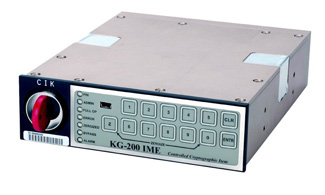
\includegraphics[width=0.33\textwidth]{inline_media_encryptor.jpg}
  \end{center}
  \caption{The $KG-200$ Inline Media Encryptor, certified by the NSA for use in securing persistent storage~\cite{nsa_ime_website}.}
\label{fig:inline_media_encryptor}
\end{figure}

\subsection{Persistent Storage}
Persistent storage as Network-Attached Storage (NAS) devices are capable of storing large quantities of user application data, and are usually of much higher capacity than the compute nodes.  These devices commonly use RAID (redundant array of inexpensive disks) technology ~\cite{katz1989disk} for higher storage efficiency and redundancy. 

It is assumed that Inline Media Encryptors (IMEs) and POSIX permissions are used to enforce data access rules within persistent storage~\cite{nsa_ime}. IMEs have been certified for use in classified networks by the U.S. National Security Administration since 2006~\cite{nsa_ime_website}. 

\subsection{Administrative Nodes}
Administrative nodes are computing devices where \begin{inparaenum}[\itshape a\upshape)]
\item both administrators and users interact with the system, common tasks of which include issuing job or system commands, accessing reports and results, and performing maintenance;
\item resource management software is centrally located and executed~\cite{keller2001anatomy}, common examples include IBM's Tivoli Workload Scheduler and the MOAB Cluster Suite by Adaptive Computing~\cite{arackal2009access}\cite{jackson2006demand}.
\end{inparaenum}

It is assumed that the scheduler located here is capable of providing access to the list of current running applications and the hardware resources devoted to them. 
\subsection{Network Infrastructure}
Network infrastructure devices facilitate the transmission of data between nodes within the HPC system. Mediums vary widely and include copper, optical, and wireless. The most common technologies used in HPC environments are Ethernet and InfiniBand~\cite{bozzo2006design}\cite{madai2010performance}. 

It is assumed that the network infrastructure uses Internet Protocol to communicate among nodes.

\subsection{Job Execution}
Best practices for developing jobs run on HPC systems dictates the minimization of I/O, both to disk and over the network ~\cite{shan2007using}. This I/O minimization is due to the dramatic increase in access time as data moves further away from the CPU and main memory. It's over 50 times more costly to access 1MB of data from the network than it is from main memory ~\cite{dean2009designs}. This overhead increases to almost a factor of 100 if that data is initially read from disk then sent over the network ~\cite{dean2009designs}.

In the effort to minimize the cost of I/O transactions, previous researchers have shown that batching I/O into larger transactions can reduce overhead~\cite{shan2008characterizing}. The difference between sequentially reading 1K files from network disks and reading 256MB from network disks shows a factor of 1700 improved performance by reading in larger batches~\cite{shan2007using}. The batching of I/O, especially the most costly forms (disk and network) is therefore considered best practice when possible~\cite{borrill2007investigation}. It is therefore assumed that job developers will attempt to maximize I/O batching, the optimal case of which would have an I/O transaction history similar to that shown in Figure \ref{fig:application_model}.

\begin{table}
	\begin{center}
	    \begin{tabular}{  l | r }
	    Action & Time to Complete \\ \hline
	    L1 cache reference & 0.5 ns  \\ 
	    L2 cache reference & 7 ns  \\
	    Main memory reference & 100 ns \\
	    Read 1 MB sequentially from memory & 250,000 ns  \\  
	    Read 1 MB sequentially from network & 10,000,000 ns \\ 
		Read 1 MB sequentially from disk & 30,000,000 ns \\
	    \end{tabular}
	\end{center}
	\caption{Access time examples showing the magnitude of difference between data over I/O and data locally stored~\cite{dean2009designs}.}
\end{table}

\begin{figure}
  \begin{center}
    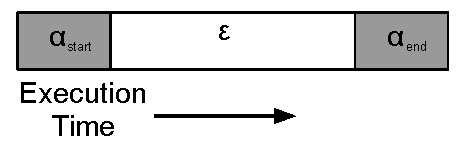
\includegraphics[width=0.48\textwidth]{application_model.pdf}
  \end{center}
  \caption{The assumed model of application execution in an HPC environment. $\alpha_{start}$ and $\alpha_{end}$ are periods where execution is I/O bound, and $\varepsilon$ is the prominent period where execution is CPU bound. This structure adheres to research showing batched I/O minimizes the I/O cost in terms of time.}
\label{fig:application_model}
\end{figure}

\section{Security Challenge}

\begin{table}
\begin{adjustwidth}{-4em}{-4em}
\centering
\begin{tabular}{ccc|c|c|}
& & \multicolumn{3}{ c }{\textbf{Solutions}} \\ \cline{3-5}
\centering\arraybackslash \textbf{Hardware Location} &  \multicolumn{1}{ c| }{\centering\arraybackslash \textbf{Security Challenge}} & \multicolumn{1}{ b{1.65cm}| }{\centering\arraybackslash Board Separation} & \multicolumn{1}{ b{.6cm}| }{\centering\arraybackslash IME} & \multicolumn{1}{ b{1.97cm}| }{\centering\arraybackslash Posix \hspace{2em}Permissions}   \\ \cline{1-5}
\multicolumn{1}{ |c| }{\multirow{2}{*}{Compute Nodes} } &
\multicolumn{1}{ |p{5cm}| }{\centering\arraybackslash Local Data Storage} & \checkmark &   & \checkmark         \\ \cline{2-5}
\multicolumn{1}{ |c  }{}                        &
\multicolumn{1}{ |p{5cm}| }{\centering\arraybackslash Local Data Processing} & \checkmark &   &  \checkmark        \\ \cline{1-5}
\multicolumn{1}{ |c|  }{Persistent Storage}  &
\multicolumn{1}{ |p{5cm}| }{\centering\arraybackslash Co-location of user data} &  &  \checkmark & \checkmark   \\ \cline{1-5}
\multicolumn{1}{ |c|  }{Administrative Node}  &
\multicolumn{1}{ |p{5cm}| }{\centering\arraybackslash Accept and Schedule User Jobs} &   &   & \checkmark   \\ \cline{1-5}
\multicolumn{1}{ |c|  }{\multirow{6}{*}{Network Infrastructure}} &
\multicolumn{1}{ |p{5cm}| }{\centering\arraybackslash Transmit intra-application data between compute nodes} &   &   &       \\ \cline{2-5}
\multicolumn{1}{ |c  }{}                        &
\multicolumn{1}{ |p{5cm}| }{\centering\arraybackslash Transmit data to/from compute nodes and persistent storage} &   &   &       \\ \cline{2-5}
\multicolumn{1}{ |c  }{}                        &
\multicolumn{1}{ |p{5cm}| }{\centering\arraybackslash Transmit commands from scheduler to compute nodes} &   &   &       \\ \cline{1-5}
\end{tabular}
\caption{Security challenges and technology used to solve them}
\label{tab:security_challenges}
\end{adjustwidth}
\end{table}

The security fear of users with extremely sensitive data is that a different user could, through chance or intention, acquire or manipulate their data. The four basic resources described above represent the resources across which data may be exposed. Table~\ref{tab:security_challenges} organizes the aforementioned ways in which these resources are secured~\cite{buyya1999high}. 

So far we have described ways in which three of the four shared resources are secured by technology that is either certified by national defense agencies (as in the case of persistent storage) or intuitive and easily verifiable (as in the case of compute node board separation and administrative POSIX permissions). This leaves the shared networking resources as a point of data sharing. 

\section{Insufficient Solutions}
\label{sec:insufficient_solutions}
There exist current solutions for the strict problem of preventing plaintext data sharing, but these solutions lack certain qualities that make them sufficient for the narrow solution we're seeking when trying to assure users assuming significant risk. These existing solutions fail through their lack of thoroughness, lack of intuitiveness, inability to be simply verified, and even through established security flaws. 
\subsection{Encryption}
Socket to socket encryption is a common solution to preventing data theft over a network, though somewhat out of place in an HPC environment due to their overhead. This solution falls short in its inability to prevent data sharing. Though the data is encrypted, the value of the plaintext (unencrypted data) is commonly so high that copying, storing and later decrypting the network traffic a risk to be prevented.
\subsection{Virtual Local Area Networks (VLANs)}
VLANs, standardized in IEEE 802.1Q~\cite{ieee_vlan}, are a common solution to preventing data sharing specifically within large computing infrastructures such as data centers and mainframes, though sometimes used in HPC environments. VLANs work by tagging traffic on network switches and routers according to configurable tables of LAN membership matched with physical interface, with the intention of mimicking the configurability and security of LANs. Within the VLAN specification there lie two inherent flaw with VLANs to verifiability that meets our envisioned users' needs, as well as a few unresolved security flaws. 

VLAN solutions are difficult to verify in two ways:
\begin{inparaenum}[\itshape a\upshape)] 
\item the logic of VLAN technology is hidden within firmware which is expensive to analyze. As VLAN technology improves and becomes more complicated, this problem will only increase in future versions of the systems~\cite{emery2011security}\cite{kloth2001derived}.
\item VLAN hardware is commonly manufactured by international firms that may have pressure from outside governments to include secret backdoors in the firmware, further exacerbating the previous verification difficulty. Examples of this uncertainty can be seen in a special report by the U.S. House of Representatives from October 8th, 2012~\cite{huawei}.
\end{inparaenum}

Furthermore, due to backwards compatibility standards outlined in IEEE 802.1Q, the tagging mechanism of VLANs can be abused via a ''double-encapsulated 802.1Q / Nested VLAN" attack which works by placing two VLAN tags on a packet. By doing so, during certain situations it is possible for packets to ''escape" their VLAN designation and convey messages to hosts outside their configured VLAN~\cite{cisco_vlan_whitepaper}.

\chapter{Design Goals}
\label{chap:design_goals}
Chapter~\ref{chap:problem_definition}'s discussion on security flaws within HPC environments shows that there exists an untouched niche for a software solution that replicates the security of physical user separation. Here we describe the requirements and goals in designing our solution to this problem.
\section{A More Thorough and Intuitive Network Security}
The gap between the security mechanisms discussed in Chapter~\ref{chap:problem_definition}: Section~\ref{sec:insufficient_solutions} and the current approach of physical user separation is large. From manufacturing and political policy problems~\cite{huawei} to simple security flaws~\cite{cisco_vlan_whitepaper}, current solutions are insufficient. For users in this domain to accept a software approach to network security in HPC environments, the proposed solution must be thorough, simple, intuitive and easily verifiable. The thoroughness of physical user separation is inherent in that it operates at the very lowest level of network operations, the physical layer. The closer our mechanism approaches this layer, the more thorough it will be considered.
\section{Dynamic Control}
Within HPC environments the type, number, and scale of jobs assigned to any of the systems can be widely varied. To handle this, the solution must be capable of receiving and modifying policy at the start of each new job. Furthermore, to manage performance tradeoffs a fine-grained control of the mechanism at higher resolution than job submission rate is desired. 
\section{Network Fabric Agnostic}
Two major technologies are used to network HPC systems: Ethernet and InfiniBand. Any tool for improving security across the broad spectrum of HPC systems must be capable of operating in each. Further, numerous network topologies exist within these technologies; switched fabric and tree structures are the most common for InfiniBand and Ethernet, respectively. For our purposes we define this solution to be network fabric agnostic if it is conceptually capable of being implemented in either Ethernet or InfiniBand networks. 
\section{User Application Transparent}
A fundamental requirement of the solution is that it be transparent to user applications. Applications written for HPC environments are often quite complex and it is likely that customers would be reluctant to make even minor modifications, especially to programs written in the past that are under re-use. For our purposes we define user application transparency as the ability to run an application without modification to successful end on an HPC system using our solution, given that it can also do so on a system not using our solution. 
\chapter{Time Division Multiple Access of Network Access}
\label{chap:tdma}
\begin{figure}
\centering
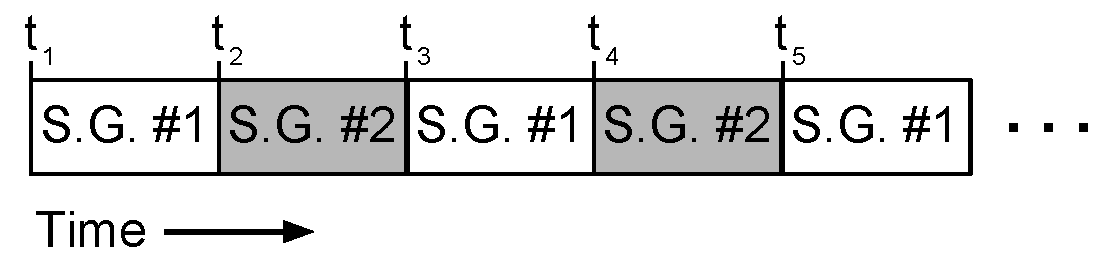
\includegraphics[scale=0.57]{network_access_slots.pdf}
\caption{A simple round-robin time window policy for two \textit{security groups} (S.G.$\#1$ and $\#2$).}
\label{fig:network_access_slots}
\end{figure}

\begin{figure}
\centering
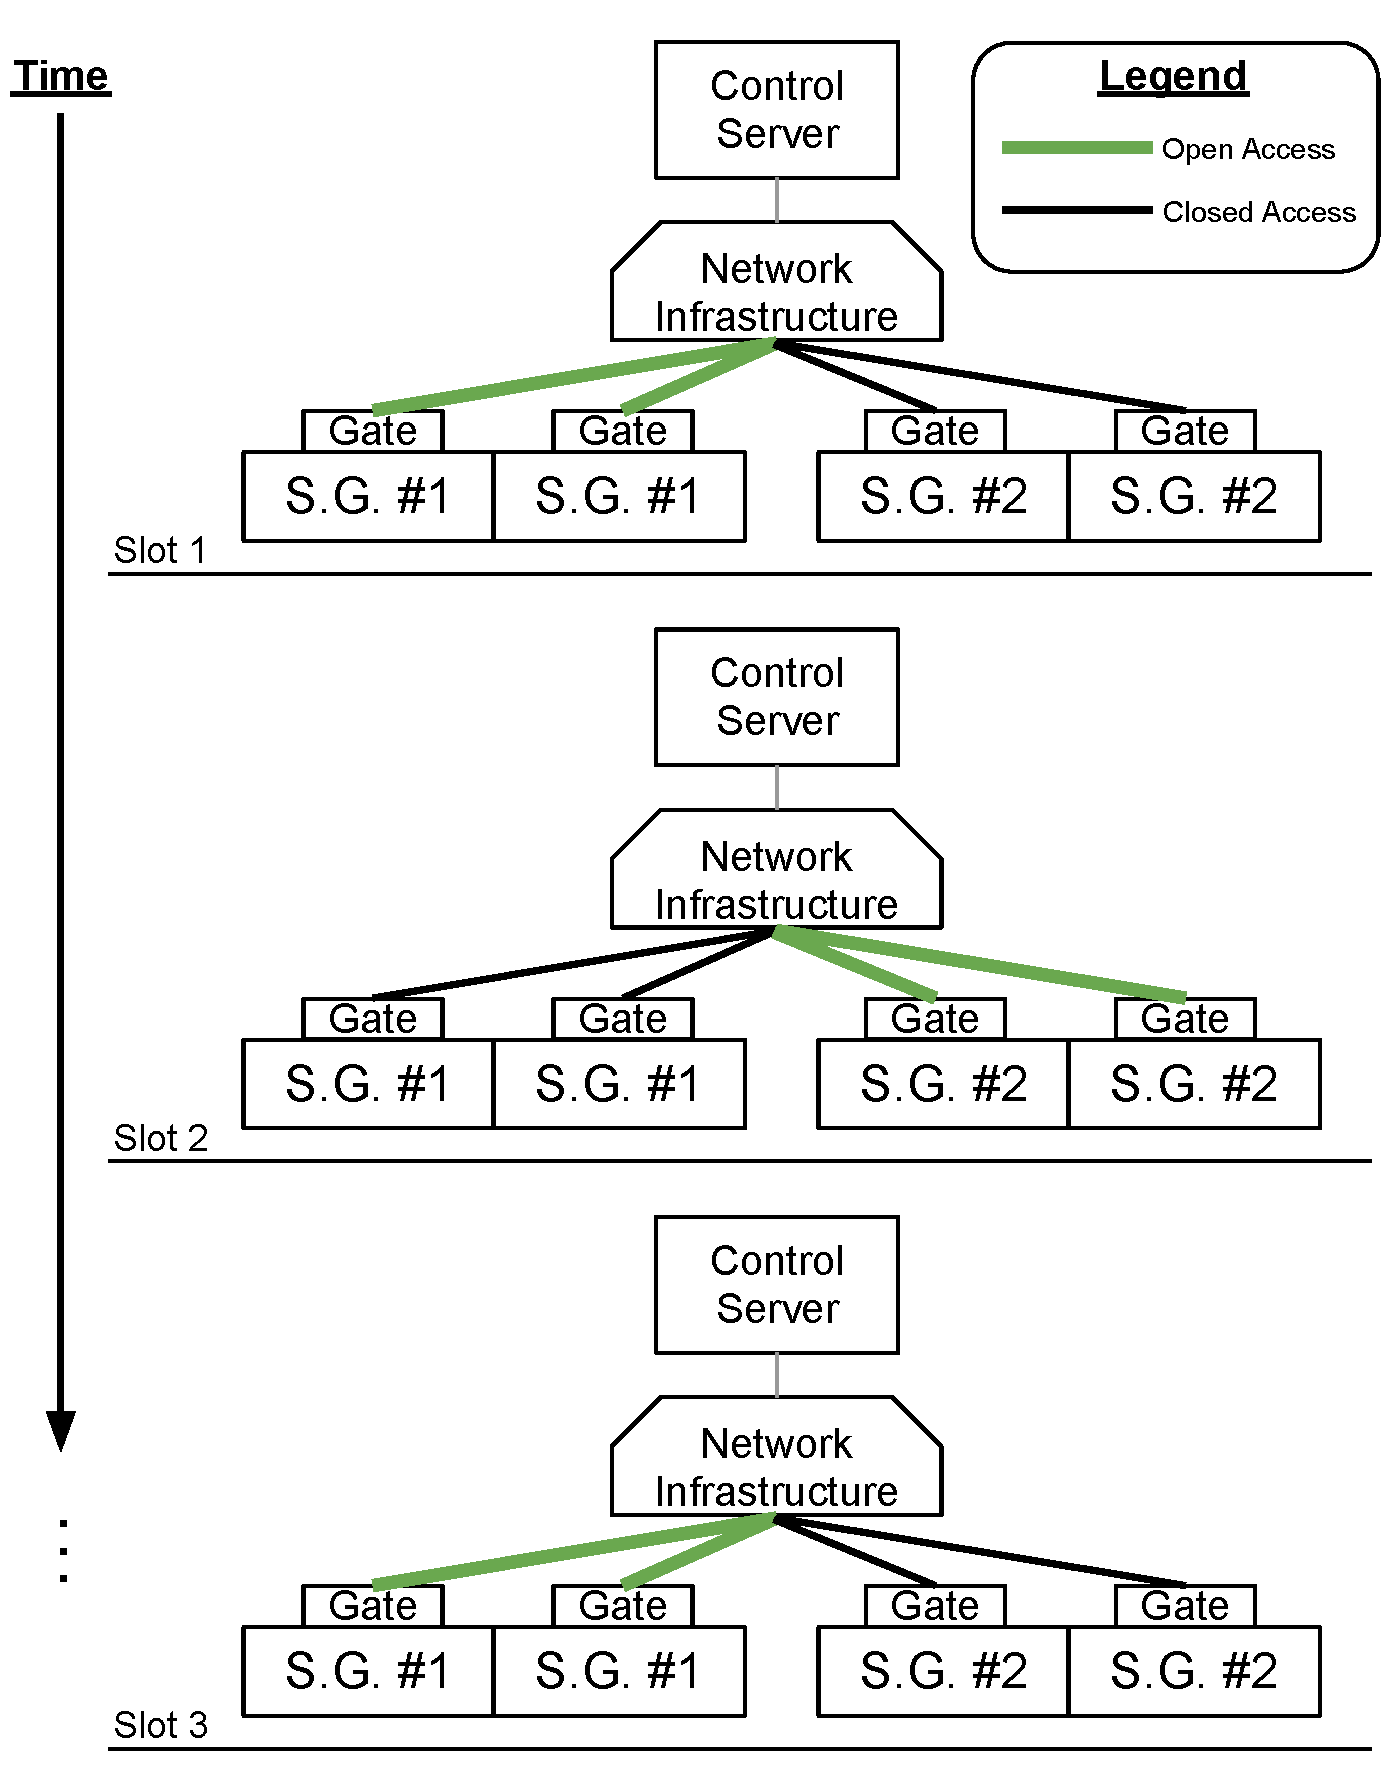
\includegraphics[scale=0.55]{network_access_switching.pdf}
\caption{A simple example of network access switching between two \textit{security groups} (S.G.$\#1$ and $\#2$).}
\label{fig:network_access_switching}
\end{figure}

The TDMA scheme introduced in Chapter~\ref{chap:introduction}: Section~\ref{sec:TDMA_intro} mimics the security of physical separation by enforcing temporal separation of network access (and denial) according to \textit{security groups}. This network access denial must be enforced at the operating system level on each compute node and controlled by the \textit{control server} which separates them into time windows. By denying disparate \textit{security groups} the ability to send or receive on the network during the same time window, both passive (packet sniffing) and active (packet insertion) data sharing are prevented.

The size and order of time windows are controlled by a scheduling policy within the \textit{control server}. Figure~\ref{fig:network_access_slots} give a simple example of a round-robin policy on two \textit{security groups}, although more complex scheduling can be created to optimize for throughput or enforce prioritization. Because the \textit{control server} modulates the opening and closing of network access at each time window, very fine grained control of scheduling policy can be achieved. It is possible to switch from round-robin scheduling during times of low network traffic to modulated window size during heavy usage by particular users, or according to whatever quality of service scheme best fits the applications. A number of heuristics are useful to consider for the creation of a dynamic priority scheduling algorithm: queue memory usage of compute nodes, number of TCP timeouts, and externally imposed priorities. 

Figure~\ref{fig:network_access_switching} shows an intuitive graphical example of network access switching between \textit{security groups} as the system passes through time windows.

\section{Formal Definition}
\label{sec:formal_definition}
Before discussing our implementation of the solution, we first define an abstract definition that describes how the mechanism works beyond any specific implementation and in a more formal way than the beginning of this chapter. The best way to describe this mechanism is through a language that represents the mechanism in operation. This language is defined formally by stating the grammar that generates it.

Suppose \emph{S} is a finite set of security groups, s.t. each security group $s\in S$ is made up of a number of compute nodes. Given \emph{S}, the language our mechanism operates on can be generated by the following grammar. Because the language is dependent on the security groups \emph{S}, this grammar must be generated based on it. This is done in two steps:

First, we define the base grammar:\\

\tab $G^1 = (V^1, \Sigma^1, R^1, \mathcal{A})$, where

\tab $V^1 = \{\mathcal{A} , W\}$ \hfill non-terminal symbols \hspace*{6em}

\tab $\Sigma ^1 = \{ \emptyset\}$ \hfill terminal symbols\hspace*{6.3em}

\tab $R^1 = \lbrace \hspace*{1.35em}\mathcal{A} \rightarrow \varepsilon ,$ \hfill rules of production \hspace*{6em} \\
$\tab \hspace*{5.9em} \mathcal{A}\rightarrow W\mathcal{A} |W\rbrace$\\

This base grammar, through the non-terminal symbols and production rules, establishes a means of generating the base language form of unordered windows ($W\in V^1$) in an arbitrary length such as $WW$ or $WWWWW$.

Next, we generate the \emph{S} specific definitions. To do so it is first necessary to define notation for two special terminal symbols and three special sets:\\
\\
$o_{s,i}$ - an open command issued to node $i$ within security group $s$,\\
$a_{s,i}$ - an acknowledgement received from node $i$ within security group $s$,\\
$\theta_s$ - the set of all $o_{s,i}$ terminals for security group $s$, \\
$\alpha_s$ - the set of all $a_{s,i}$ terminals for security group $s$, and \\
$\pi(A)$ - the set of all permutations of the set A.\\

These definitions allow us to define a final, special set:\\
\\
$\Lambda_s = \pi(\theta_s) \times \pi(\alpha_s)$\\

Intuitively, $\Lambda_s$ is a set of ordered sets expressing each permutation of $\theta_s$ matched with each permutation of $\alpha_s$. For example, given a security group $s$ made up of two elements s.t. $s = \{1, 2\}$, $\Lambda_s$ is defined:\\
\\
$\Lambda_s = \{ (o_{s,1}, o_{s,2}, a_{s,1}, a_{s,2}),\hspace*{1.0em} (o_{s,2}, o_{s,1}, a_{s,1}, a_{s,2}),$\\
\hspace*{3.0em}$ (o_{s,1}, o_{s,2}, a_{s,2}, a_{s,1}),\hspace*{1.0em} (o_{s,2}, o_{s,1}, a_{s,2}, a_{s,1})\}$\\

The sets within $\Lambda_s$ represent all legitimate command sequences within a window ($W$) for security group $s$. The key property of the sets within $\Lambda_s$ is that each node within the security group is issued an open command, in any order, followed by acknowledgements from each node within the security group, once again in any order.

With these definitions established we can now formally define an $\emph{S}$ specific grammar:

\tab $G^2 = (V^2, \Sigma^2, R^2, \emptyset)$, where

\tab $V^2 =\{W\}$

\tab $\Sigma ^2 = \{[o_{s,i}, a_{s,i}]:\forall i \in \forall s\in \emph{S}\}$

\tab $R^2 = \{[W\rightarrow \lambda  ] :\forall \lambda \in \Lambda_s :\forall s\in \emph{S}\}$


These definitions add new terminal symbols and the necessary production rules to generate them. Note the use of $\Lambda_s$ in the production rules. These rules provide every possible command sequence possible for any window $W$ s.t. every node issued an open command is required to report back with an acknowledgement before continuation onto another window.

Finally, the language our mechanism accepts for security group \emph{S} can be formed using the union of the previous two grammars:\\

\tab $G = (V, \Sigma , R, \mathcal{A})$, where

\tab $V = V^1\cup V^2$

\tab $\Sigma = \Sigma ^1\cup \Sigma ^2$

\tab $R = R^1\cup R^2$
\chapter{Implementation}
\label{chap:implementation}
As a proof of concept we have implemented a version of the tool for the Linux operating system using C++11. In this section we will describe the tool's architecture, operation, and how it adheres to the design goals from Chapter~\ref{chap:design_goals}.
\section{Overview}
The tool is composed of four major components:  the control server, ingress controller, egress controller, and the state controller. The control server can be located on any administrative node within the system, preferably co-located with the system job scheduler. The remaining controllers are located throughout the HPC environment, with a copy on each compute node that is designated to execute user applications. 

As jobs are scheduled on the system, the control server must be informed of the Internet Protocol, or IP, addresses assigned to that application and the assigned security group. As jobs are run on compute nodes throughout the system the control server communicates with the state controller on each node to designate time windows. This communication is sent via a standard TCP communications socket. For any given time window in which a security group does not have access to the network, outgoing network packets are stored in a local queue while incoming packets not sourced according to a ``whitelist" firewall are ignored and deleted. The control server is tasked with alternating time window authorization between security groups.

The following subsections describe each components operations in further detail. 
\section{State Controller}
The state controller has four major tasks:
\begin{enumerate} \itemsep1pt \parskip0pt \parsep0pt
\item Securely send and receive communication with the control server including receiving open network access commands and sending acknowledgements that the ingress and egress controllers have been transitioned to a state of network denial (closed).
\item Transit both the ingress and egress controllers between states of network access and denial.
\item Track time for which it must issue state transitions and communications with the control server.
\item Collect and store performance data on the egress queue's memory usage.
\end{enumerate}

A state machine of the state controller is shown in Figure~\ref{fig:node_state_diagram}. For a detailed algorithm of the state controller see Algorithm~\ref{alg:state_controller} in Appendix~\ref{app:tdma_algorithms}.

\begin{figure}
\centering
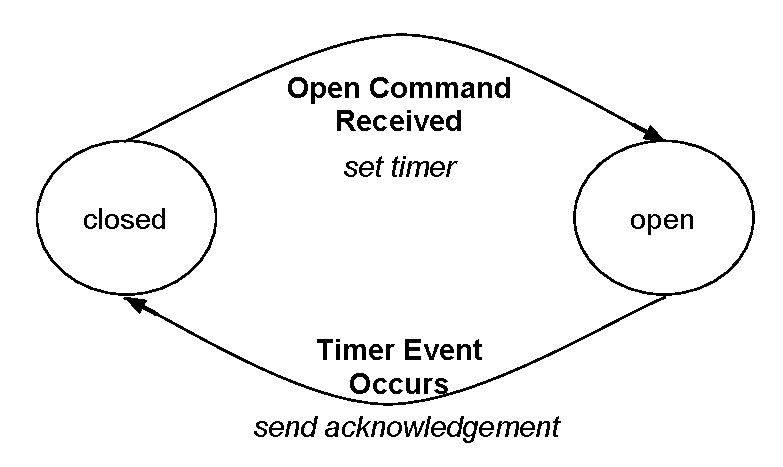
\includegraphics[scale=0.7]{node_state_diagram.pdf}
\caption{State diagram of a compute node running the state controller.}
\label{fig:node_state_diagram}
\end{figure}

\section{Ingress and Egress Controllers}
The ingress and egress controllers are firewall rules created and manipulated by the state controller. The rules are implemented using \textit{iptables} and \textit{NetFilter}, the packet filtering firewall technology that has come standard with the Linux kernel since version 2.4~\cite{iptables}. These controllers occur in two states, network access and network denial. When in the network access state, they are to allow network packets to flow freely to and from local applications. When in the network denial state each controller has a specific task: 

\begin{enumerate}
\item The ingress controller must deny and drop all network packets received except those specifically allowed according to a whitelist. This whitelist is specifically issued by the control server at the beginning of execution, and dictates the IP and MAC address of administrative services within the environment from which communication must not be broken. Example of such services include Network Time Protocol, resource scheduling communication, and the control server itself must have an entry in this whitelist.
\item The egress controller must enqueue outgoing packets exempting those specifically allowed through according to the aforementioned whitelist. These packets must be stored in main memory in preparation for transmission once network access is again granted.
\end{enumerate}

When these controllers transition out of the network denial state, a certain protocol must be followed in order to avoid the system dropping packets. All nodes within the security group to which a state of network access is now being issued must transition their ingress controllers before any single node within the group transitions their egress controllers. The reason simply being that upon transitioning egress controllers into the network access state, they will begin transmitting (in a first-come first-served order) the packets sitting in their queue. If nodes within that security group have yet to transition their ingress controller, packet arrivals sourced from within their own security group would be dropped as if they were sourced outside the security group.

\subsection{iptables and NetFilter}
\begin{figure}
\centering
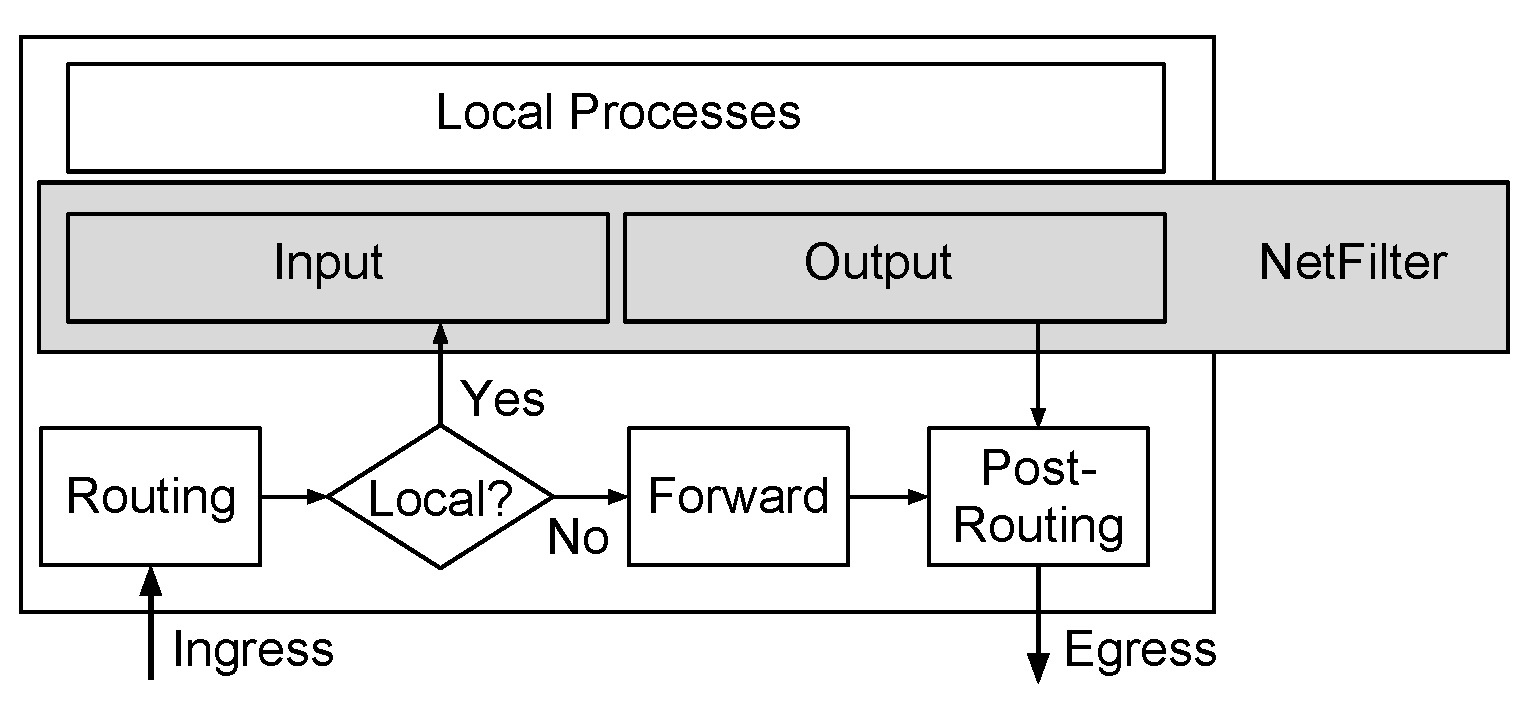
\includegraphics[scale=0.55]{netfilter_chain.pdf}
\caption{Data flow architecture of \textit{iptables}, the packet filtering firewall with \textit{NetFilter} located within the Linux kernel. The input and output ''chains" within \textit{NetFilter} provide an interface for administrators to control and filter packets sent into user space.}
\label{fig:netfilter_chain}
\end{figure}

Figure~\ref{fig:netfilter_chain} provides a concise overview of the components within \textit{iptables}. With \textit{iptables} enabled, all packets sent and received from the operating system are passed through a series of checks. At each check, \textit{iptables} is capable of transforming the data within that packet according two edicts
\begin{inparaenum}[\itshape a\upshape)] 
\item routing tables and
\item \textit{NetFilter} chains
\end{inparaenum}
before data is delivered from the network to local processes and before local processes can deliver packets to the network medium.

It is within \textit{NetFilter} that the logic of the ingress and (most of the) egress controllers are located. Within \textit{NetFilter}'s input and output processes administrators can insert ``chains" of logic to redirect the flow or, or manipulate the contents of packets. Figure~\ref{fig:netfilter_in_out_chains} provides a visual summary of the ingress and egress controller logic located within \textit{NetFilter} as chains. 

The queue structure in Figure~\ref{fig:netfilter_in_out_chains}'s output section is controlled by the egress controller registering a special subroutine to process the packets when in the network access state. This subroutine is registered using \textit{NetFilter}'s \textit{$libnetfilter\_queue$} library~\cite{libnetfilterqueue}.

\begin{figure}
\centering
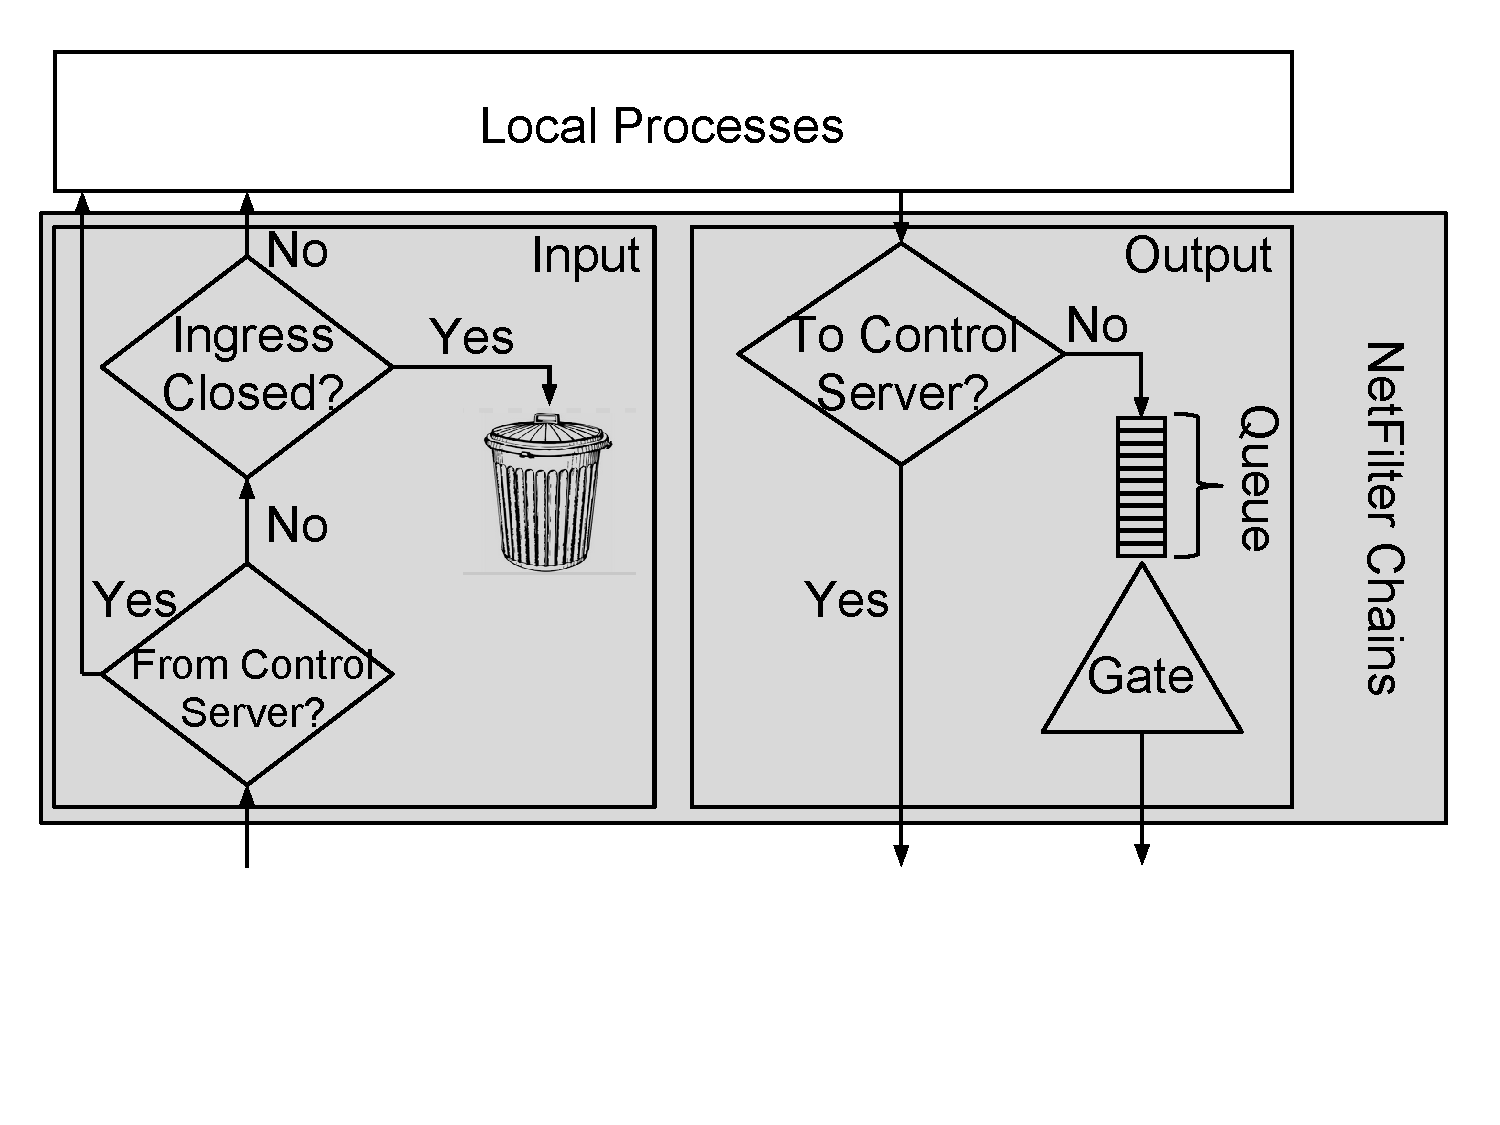
\includegraphics[scale=0.57]{netfilter_in_out_chains.pdf}
\caption{A detailed look at the logic within the \textit{NetFilter} chains that makeup the Ingress and Egress controllers on compute nodes.}
\label{fig:netfilter_in_out_chains}
\end{figure}

\section{control server}
The control server has three major tasks: 
\begin{enumerate}
\item Determine system network access states for the next time window.
\item Validate the closure of the previous time window.
\item Communicate the next time window states to compute nodes.
\end{enumerate}

To determine the network access states for the next time window the scheduler must run a scheduling algorithm on a few historical inputs. A state machine of the control server is shown in Figure~\ref{fig:control_state_diagram}. The control server transitions between states of open network access for individual security groups. During these states the control server waits to receive acknowledgement from the state controllers of that security group showing network access denial has been enforced for all nodes of the group. 

For a detailed algorithm of the control server see Algorithm~\ref{alg:control_server} in Appendix~\ref{app:tdma_algorithms}.



\begin{figure}
\centering
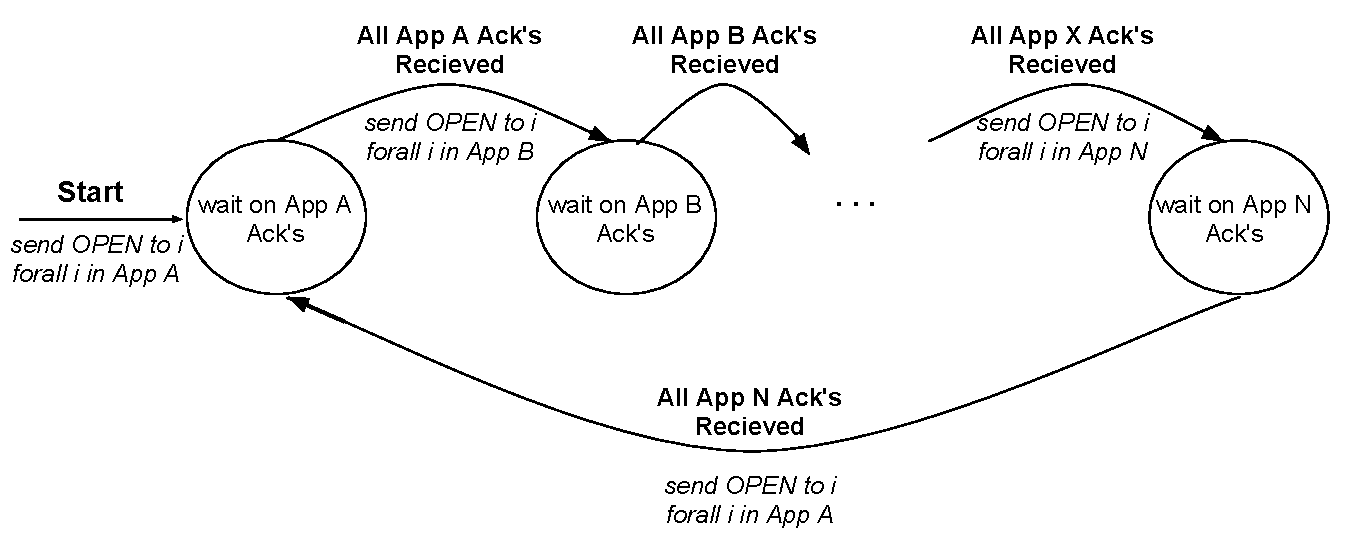
\includegraphics[scale=0.62]{control_state_diagram.pdf}
\caption{State diagram of an example window controller.}
\label{fig:control_state_diagram}
\end{figure}


\chapter{Performance}

\begin{figure}
\centerline{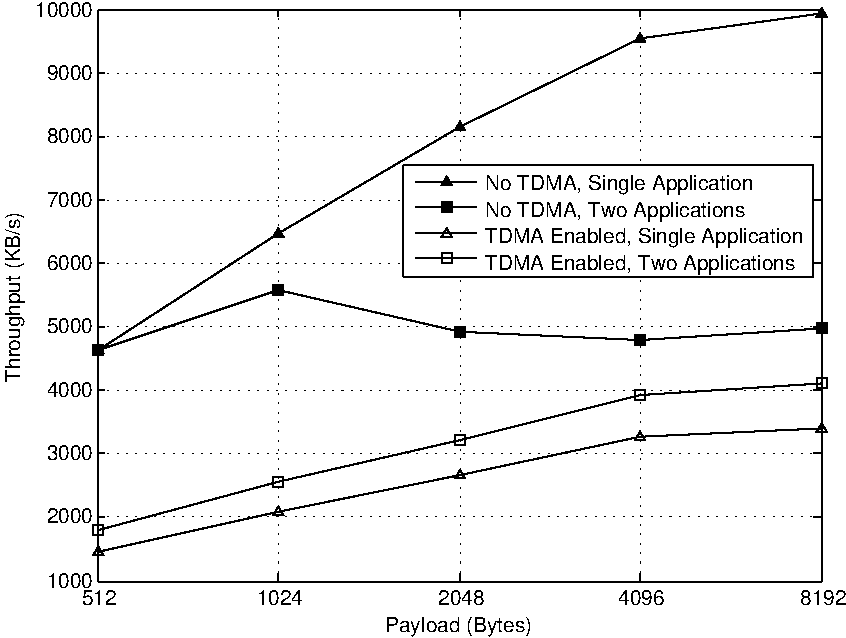
\includegraphics{TCP_Performance.pdf}}
\caption{TDMA effect on TCP application performance and demonstration of payload size effect on network throughput.}
\label{fig:TCP_Performance}
\end{figure}

\begin{figure}
\centering
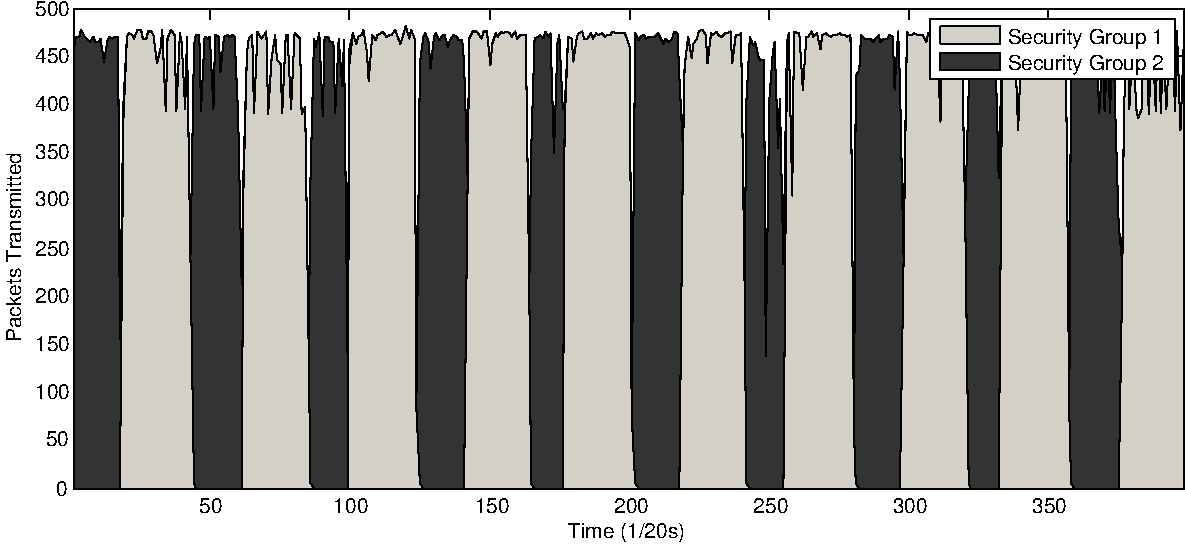
\includegraphics[scale=0.8]{Switching.pdf}
\caption{A trace of network traffic under performance testing while TDMA controls access.}
\label{fig:Switching}
\end{figure}

\begin{figure}
\centering
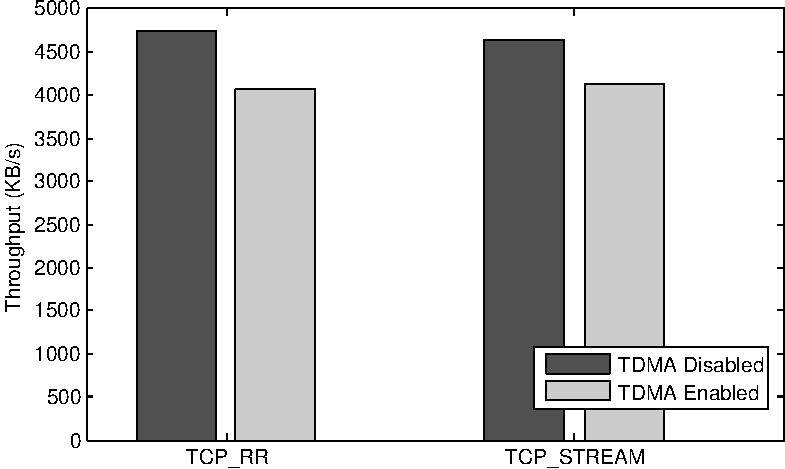
\includegraphics[scale=0.75]{detailed_performance.pdf}
\caption{The impact of TDMA on TCP performance under two different 'netperf' tests.}
\label{fig:detailed_performance}
\end{figure}

\section{Expected Values}

\begin{table}
	\begin{center}
	    \begin{tabular}{  l | r  }
	    Technical Specifications & \\ \hline
	    CPUs & 16 cores @ 2.2GHz \\
	    Main Memory & 32GB @ DDR3\\
	    \end{tabular}
	\end{center}
	\caption{Technical specifications of compute nodes within the Titan at ORNL.}
	\label{tab:titan_ORNL}
\end{table}
MAKE SURE TO CITE NETPERF~\cite{netperf}
Leading systems in high performance computing can serve as indicators of where commercial HPC systems will be in the upcoming years. The Titan system at Oak Ridge National Laboratories (ORNL) is one such system, the technical details of which are displayed in Table~\ref{tab:titan_ORNL}.

Here we attempt to quantify how the mechanism affects memory usage at the compute node level and effective bandwidth.
\begin{description}
    \item[$T_{on, n}$] Time, within a window, where compute node $n$ has access to the network.
    \item[$T_{window}$] Length in time of a single window.
    \item[$\Pi_{app, n}$] Speed at which the application on compute node $n$ generates network traffic.
    \item[$\Pi_{NIC, n}$] Speed at which the NIC on compute node $n$ can transmit traffic onto the network.
\end{description} 

\section{Case Study}
To verify and test the mechanism a test bed was created out of five Dell $1955$ servers seen in Figure~\ref{fig:test_bed}. These servers run Ubuntu server version 12.04 and had their network interfaces configured and connected according to Figure~\ref{fig:tdm_demo_setup}. 

To simulate job execution each node ran a program that sent ICMP (ping) commands at stochastic intervals and speeds to the other member other member of the security group. The mechanism, started and controlled at the control server (see Figure~\ref{fig:test_bed}) alternated between network access for each security group at a time interval of one second of network access per group. A Wireshark (REF PACKET SNIFFING) trace was ran at the control server and the results of which can be seen in Figure~\ref{fig:wireshark} showing a history of packets sent through the network. The black entries represent communications originating from the control server, while the red and blue entries represent packets originating from nodes within the security group. [REMOVE MAKE IMAGE OF RANDOMIZED PINGING AND COMPARE THE BEFORE AFTER - MENTION THIS IS EGRESS INFORMATION, FIND WAY TO SHOW INGRESS.]
\begin{figure}
  \begin{center}
    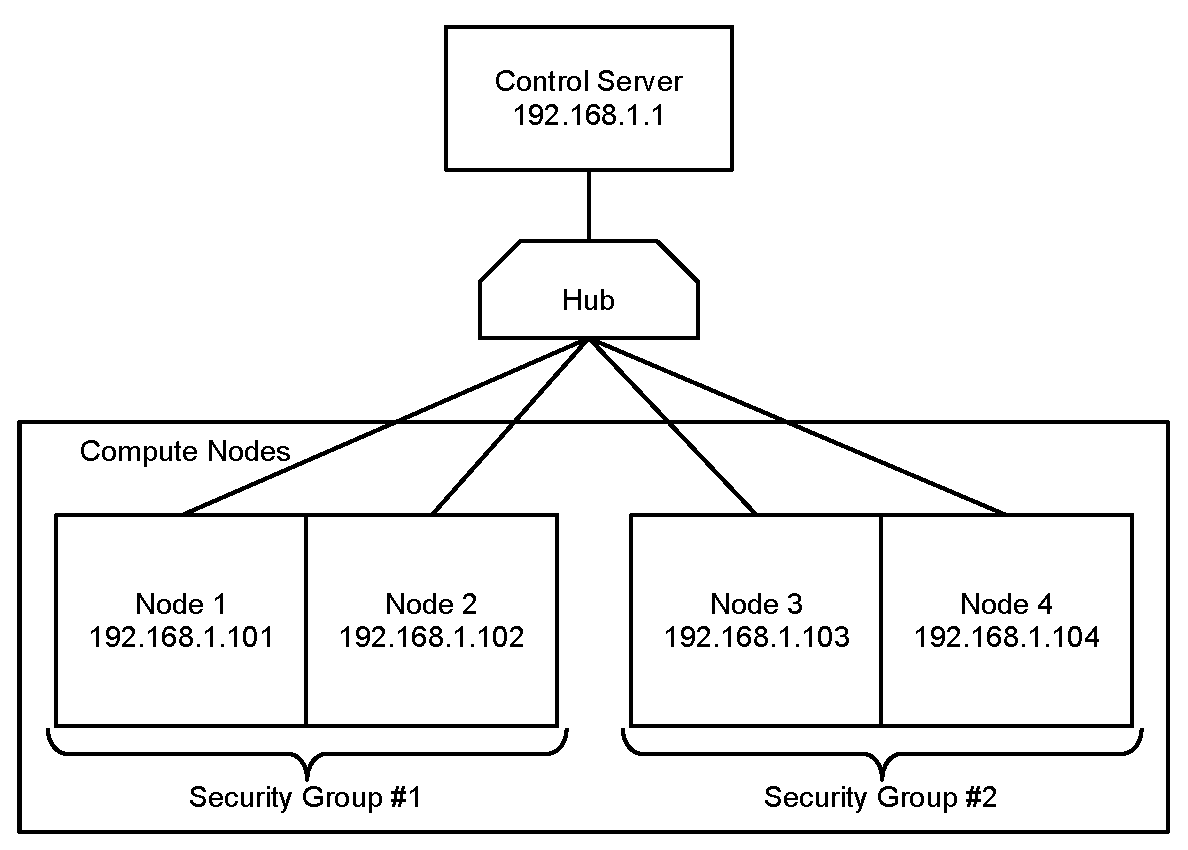
\includegraphics[width=0.9\textwidth]{tdm_demo_setup.pdf}
  \end{center}
  \caption{The network architecture of our demonstration test bed.}
\label{fig:tdm_demo_setup}
\end{figure}

\begin{figure}
  \begin{center}
    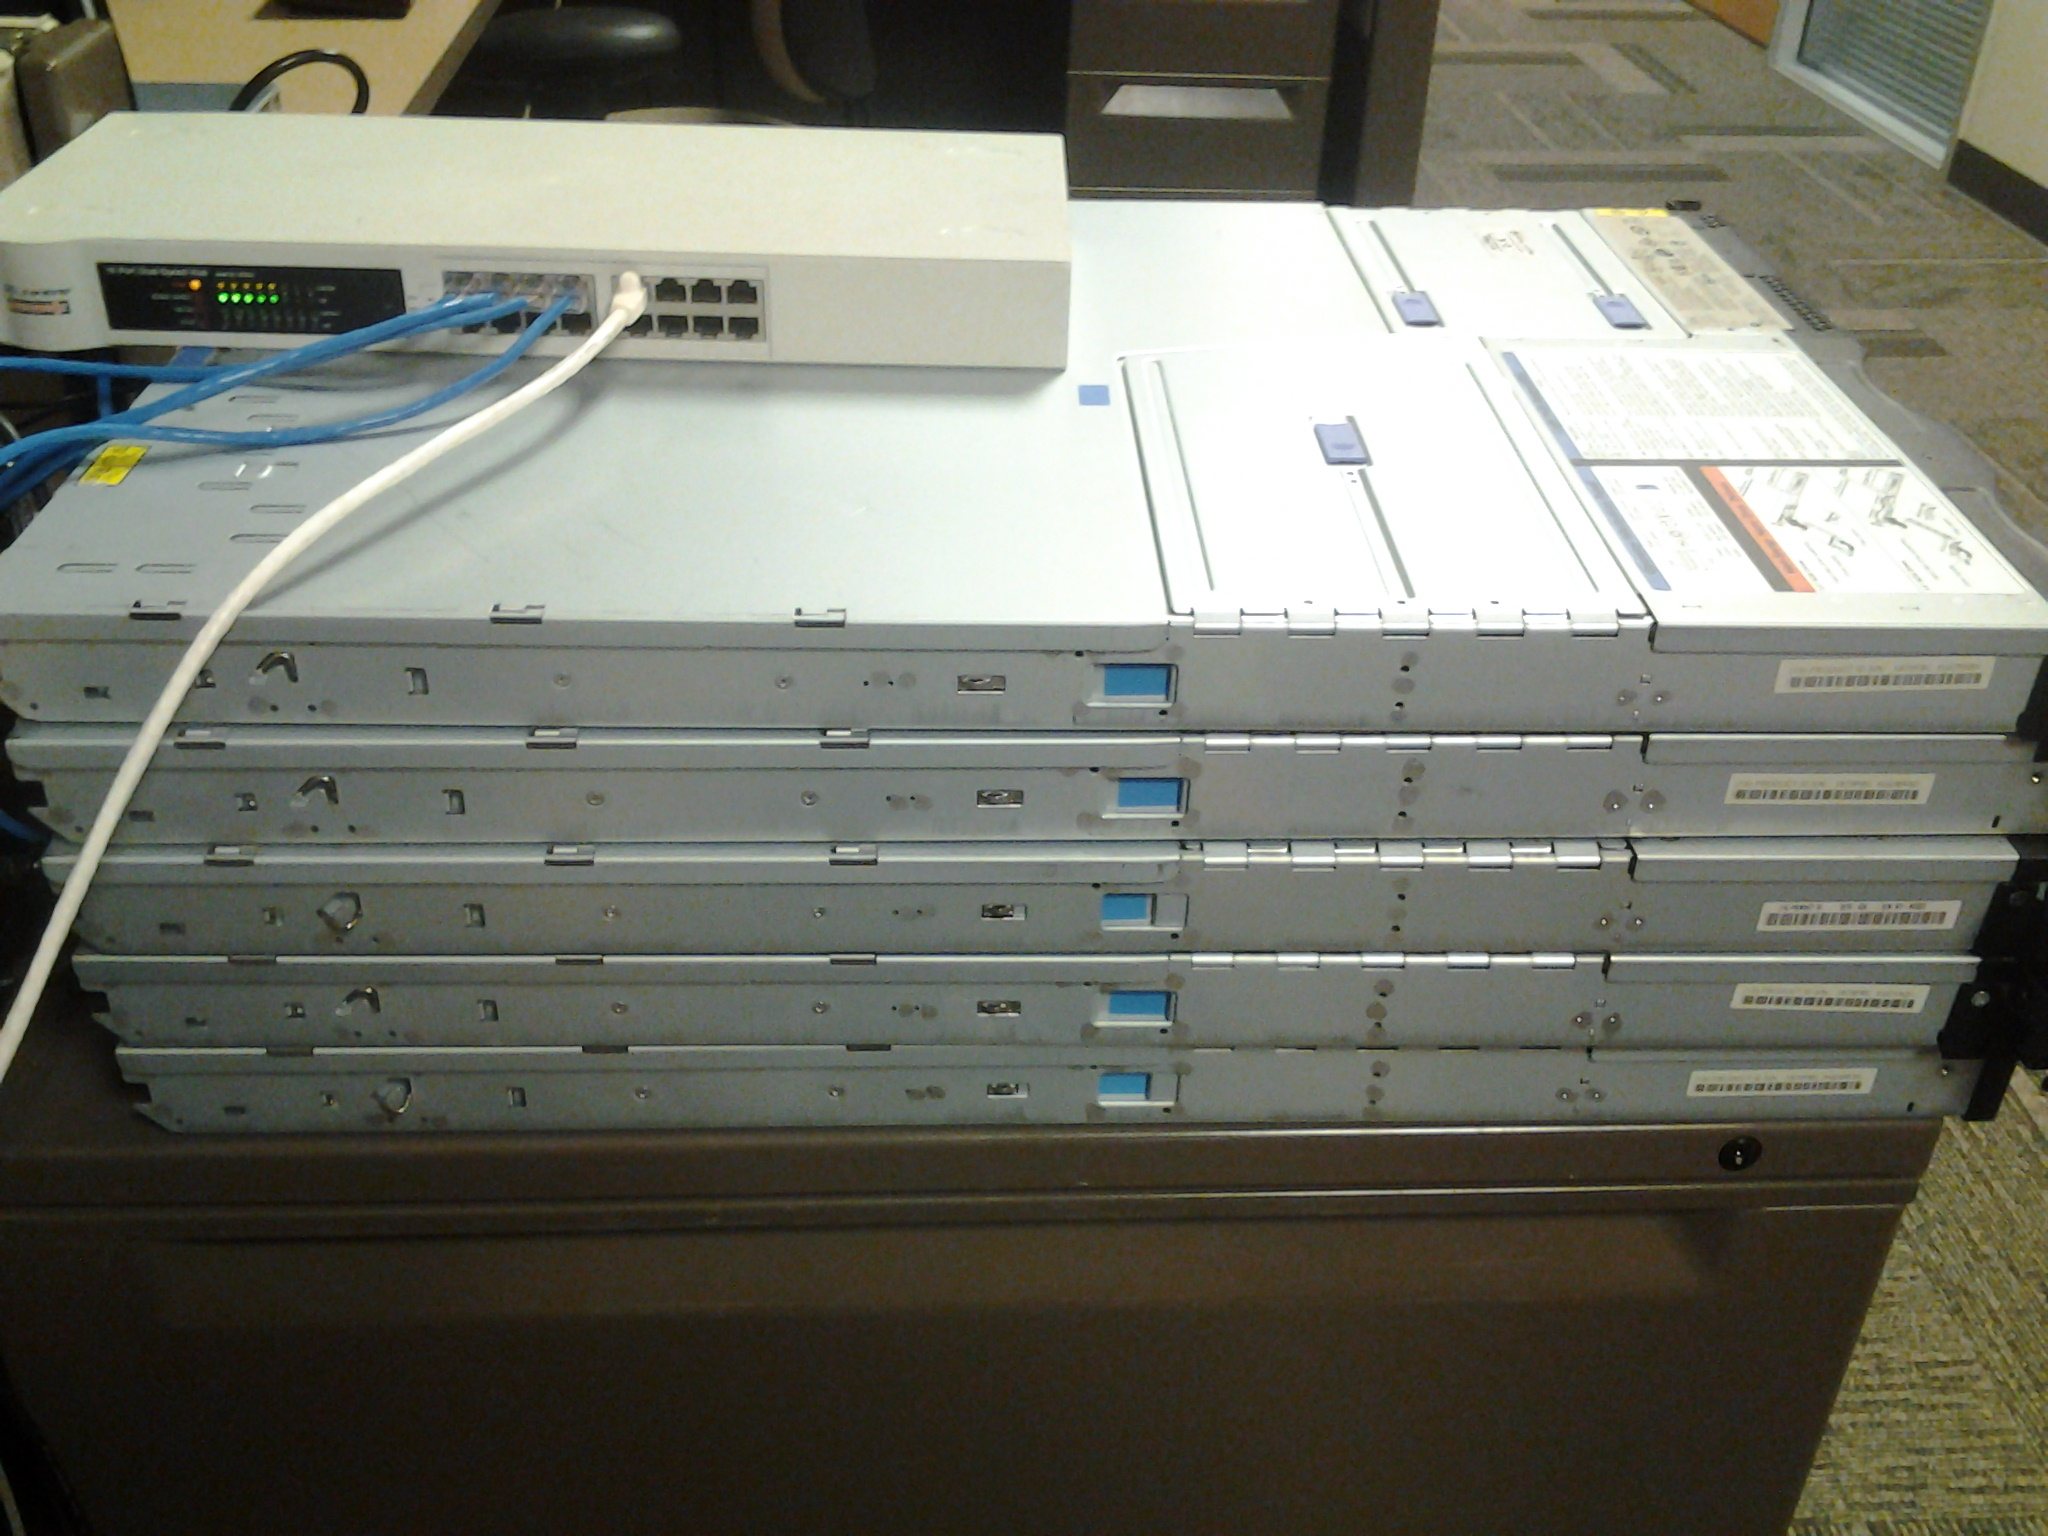
\includegraphics[width=0.9\textwidth]{test_bed.jpg}
  \end{center}
  \caption{The TDMA test bed located in Impact Lab at Arizona State University.}
\label{fig:test_bed}
\end{figure}
    
    
\begin{figure}
  \begin{center}
    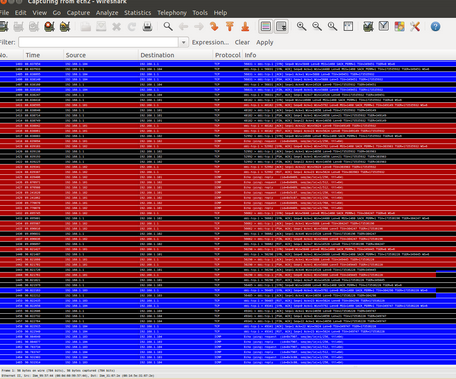
\includegraphics[width=0.9\textwidth]{wireshark.jpg}
  \end{center}
  \caption{An example trace of the mechanism's time division property captured using the packet capturing application Wireshark. The colored records represent traffic based from compute nodes of two separate security groups - denoted as red and blue.}
\label{fig:wireshark}
\end{figure}

\begin{figure}
  \begin{center}
    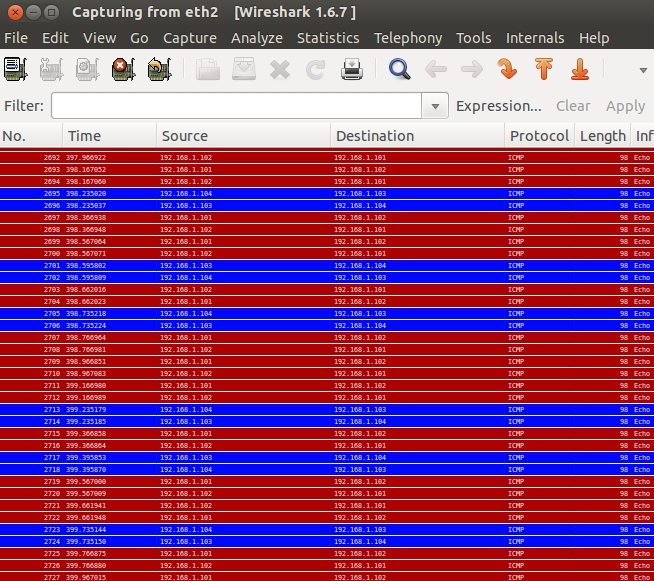
\includegraphics[width=0.9\textwidth]{wireshark_random.jpg}
  \end{center}
  \caption{An example trace of applications operating without TDMA. Note the interweaving of traffic from the different security groups - denoted as red and blue.}
\label{fig:wireshark_random}
\end{figure}

\section{Security Validation}
\chapter{Conclusion}
The problem of enforcing authenticated access to resources in an HPC environment is a difficult one. Further, creating a solution that is intuitive and secure enough to convince highly sceptical stakeholders of its security narrows available options. This thesis presents a method of solving this problem that is both intuitive and verifiably secure, in real time. The worst case performance penalty of utilizing this mechanism is shown to be within bounds of reasonable expectations. Practical performance is expected to minimize the overhead of the mechanism. 
\section{Further Work}
Implement dynamic scheduling algorithm on the control server using memory usage statistics from compute nodes. 
\appendix
\chapter{Implemented TDMA Algorithms}
\label{app:tdma_algorithms}
\begin{algorithm}
	\caption{Control Server opening and closing network access windows.}
	\label{alg:control_server}
	\begin{algorithmic}[1]
	\Statex
	\Function{$Open\_Windows$}{$Scheduler$}
		\State $Scheduler.initialize();$
		\While{$End\_Command\_Not\_Received$}
			\State $Security\_Group \gets Scheduler.get\_next\_group();$
			\State $Security\_Group.state \gets \textsc{state.open};$
			\ForAll {$node \in Security\_Group$}
				\State $send(node.address,$ \par
	        \hskip\algorithmicindent\hspace{3em} $Security\_Group.crypto\_sign(\textsc{command.open}));$
        \State $node.state \gets \textsc{state.open};$
			\EndFor
			\While{$Security\_Group.state == \textsc{state.open}$}
				\State $node\_response \gets block\_on\_receive\_message();$
				\If{$node\_response.state == \textsc{state.closed}$} 
					\State $node.state \gets \textsc{state.closed};$
				\Else 
					\State $\textbf{throw}\hspace{.6em} \textsc{error.unclosed\_node};$
				\EndIf
				\State $Security\_Group.state \gets \textsc{state.closed};$
				\ForAll {$node \in Security\_Group$}
					\If{$node.state == \textsc{state.open}$}
						\State $Security\_Group.state \gets \textsc{state.open};$
					\EndIf
				\EndFor
				
			\EndWhile
		\EndWhile

	\EndFunction

	\end{algorithmic}
\end{algorithm}

\begin{algorithm}
	\caption{State Controller Mechanism opening and closing network access to nodes by security group.}
	\label{alg:state_controller}
	\begin{algorithmic}[1]
		\Statex
		\Function{$Node\_Control\_Mechanism$}{}
			\State $Queue \gets initialize\_queue;$
			\While{$exit\_command\_not\_received$}
				\State $state \gets Close\_Network\_Access(Queue);$
				\While {$open\_command\_not\_received$}
					\State $message \gets block\_on\_receive\_message();$
				\EndWhile
				\State $state \gets Open\_Network\_Access(Queue);$
				\State $sleep(message.time);$
				\State $state \gets Close\_Network\_Access(Queue);$
				\State $send\_acknowledgement(state);$
			\EndWhile
		\EndFunction
		\Statex
		\Function{$Close\_Network\_Access$}{$Queue$}
			\State $state.egress \gets Network\_Egress.enqueue(Queue);$
			\State $state.ingress \gets Network\_Ingress.drop\_packets();$
			\State \Return{$state$}
		\EndFunction
		\Statex
		\Function{$Open\_Network\_Access$}{$Queue$}
			\State $state.ingress \gets Network\_Ingress.accept\_packets();$
			\State $state.egress \gets Queue.process\_packets\_to\_network();$
			\State \Return{$state$}
		\EndFunction
	\end{algorithmic}
\end{algorithm}	
\bibliographystyle{plain}
\bibliography{bibliography}

\end{document}
